\chapter{Diagramma delle velocità}
Il diagramma delle velocità è la rappresentazione grafica dell'andamento della velocità di progetto in funzione della progressiva dell'asse stradale. Si costruisce, sulla base del solo tracciato planimetrico, calcolando per ogni elemento di esso l'andamento della velocità di progetto, che deve essere contenuta nei limiti inferiori e superiori per le velocità di progetto degli elementi planoaltimetrici che compongono il suo asse.
\leavevmode\\
Per creare il diagramma delle velocità si usa il comando Geometry/italian checks/speed diagram impostando la normativa italiana e la tipologia di strada, F extraurbana nel nostro caso, e la velocita massima di progetto. Successivamente basterà cliccare sulla sopraelevazione per ottenere il diagramma (\ref{Diagramma delle velocità}).

\begin{figure}[H]
    \includegraphics[width=\textwidth]{Figures/Diagramma delle velocità.png}
      \caption{Diagramma delle velocità}
      \label{Diagramma delle velocità}
\end{figure}

Ottenuto il diagramma delle velocità e il profilo dei cigli si può procedere con la verifica  dei criteri di Normativa utilizzando il comando Geometry/Italian checks/orizontal vertical checks.

\begin{figure}[H]
    \includegraphics[width=\textwidth]{Figures/Controllo delle velocità.png}
      \caption{Controllo delle velocità}
      \label{Controllo delle velocità}
\end{figure}

\begin{figure}[H]
    \centering
      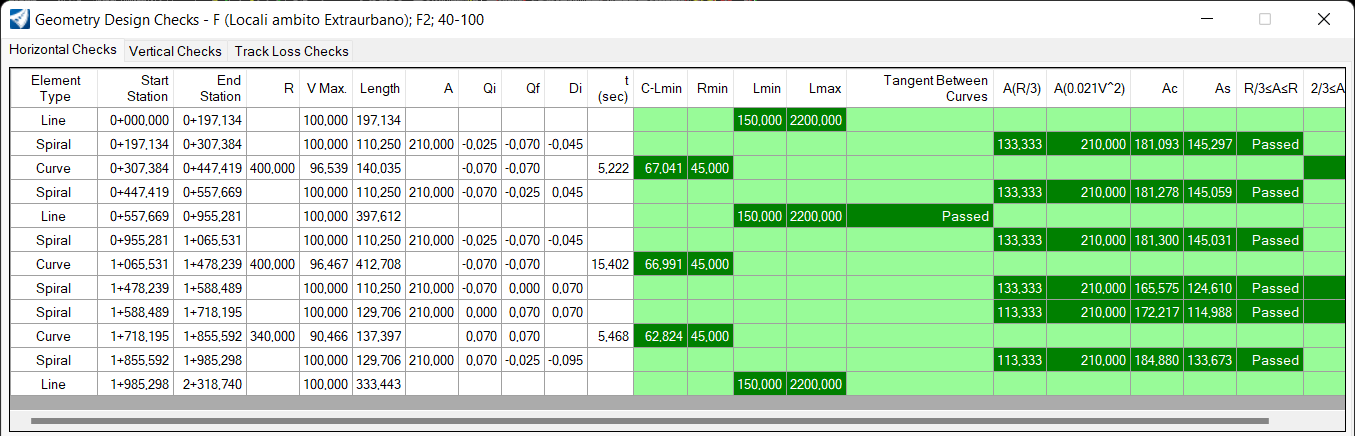
\includegraphics[width=\textwidth]{Figures/Controllo planimetrico.png}
      \caption{Controllo planimetrico}
      \label{Controllo planimetrico}
\end{figure}

\begin{figure}[H]
      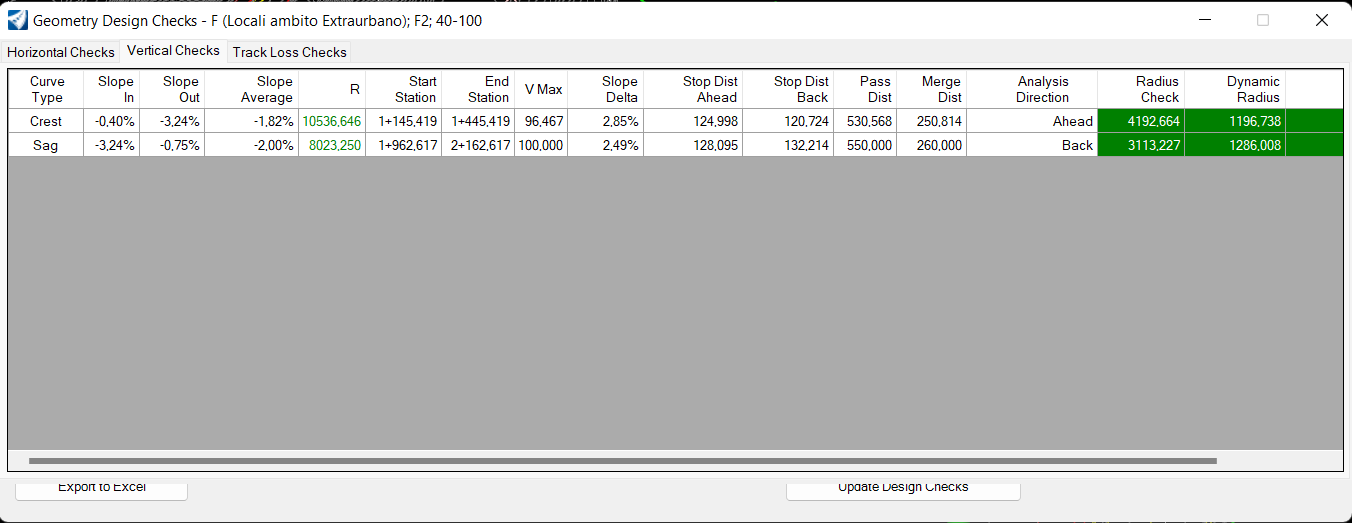
\includegraphics[width=\textwidth]{Figures/Controllo altimetrico.png}
      \caption{Controllo altimetrico}
      \label{Controllo altimetrico}
  \end{figure}

  \begin{figure}[H]
    \centering
      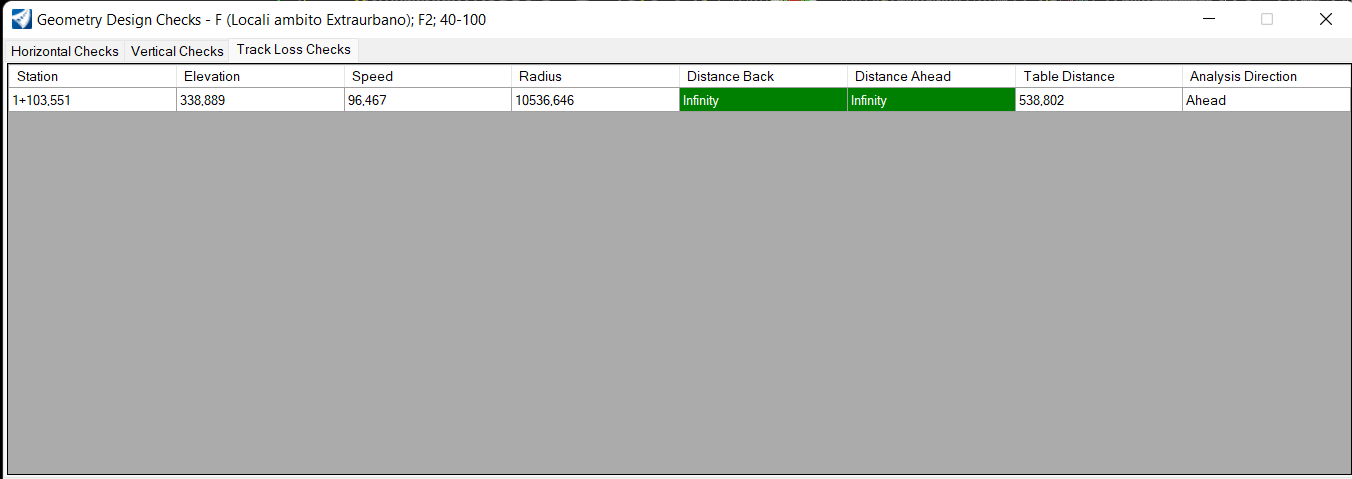
\includegraphics[width=\textwidth]{Figures/Perdita di tracciato.png}
      \caption{Perdita di tracciato}
      \label{Perdita di tracciato}
    \end{figure}

    Possiamo calcolare e verificare anche le visibilità attraverso il comando Terrain/Sight Visibility :

    \begin{figure}[H]
      \includegraphics[width=\textwidth]{Figures/Visibilità.png}
      \caption{Visibilità}
      \label{Visibilità}
  \end{figure}